% Page Layout
\documentclass[12pt,t]{beamer}
\usepackage{etex} % Avoid an error due to a lack of registers
\usepackage[english]{babel} % Defines the language of macros as well
\usepackage{float}
\usepackage{amsmath}
\usepackage{listings}
\usepackage{geometry}
\usepackage{graphicx}
% Desired Packages
%\usepackage[pdftex]{graphicx}
\usepackage[utf8]{inputenc}
\usepackage{amsmath}
\usepackage{amssymb}
\usepackage{lastpage}
\usepackage{listings}
\usepackage{caption}
\usepackage{xy}
\usepackage{microtype}
\usepackage{lmodern, hfoldsty}
\usepackage{ellipsis}
\usepackage{tabularx}
\usepackage{beamerthemeshadow}
\usepackage{nameref}
\usepackage{hyperref}
\usepackage{subfig}
\usepackage[absolute,overlay]{textpos}
\setlength{\TPHorizModule}{\paperwidth}
\setlength{\TPHorizModule}{\paperheight}

% Further Configurations
\newcommand{\Fat}[1]{{\large \bf \textcolor{cdc_Blue}{#1}}}
\renewcommand\rmdefault{pmy}            		% Activate Myriad Font
\definecolor{Gray}{rgb}{0.5, 0.5, 0.5}  		% Define light color
\definecolor{HighlightRed}{rgb}{0.6, 0.0, 0.0}  % Define light highlighting color
\graphicspath{{images/}}
\usetheme{UniOldbg}                     		% The main thing: our theme



\title[WPMP - Energy Meteorology]{WPMP - Energy Meteorology}
\author[Jan \& Florian]{Jan Kämper \& Florian Börgel}
\date{\today}
\semester{Semester 2016}
\institute{Universität Oldenburg}

\begin{document}

\definecolor{mygreen}{rgb}{0,0.6,0}
\definecolor{mygray}{rgb}{0.5,0.5,0.5}
\definecolor{mymauve}{rgb}{0.58,0,0.82}

\lstset{ %
  backgroundcolor=\color{white},   % choose the background color; you must add \usepackage{color} or \usepackage{xcolor}
  basicstyle=\footnotesize,        % the size of the fonts that are used for the code
  breakatwhitespace=false,         % sets if automatic breaks should only happen at whitespace
  breaklines=true,                 % sets automatic line breaking
  captionpos=b,                    % sets the caption-position to bottom
  commentstyle=\color{mygreen},    % comment style
  deletekeywords={...},            % if you want to delete keywords from the given language
  escapeinside={\%*}{*)},          % if you want to add LaTeX within your code
  extendedchars=true,              % lets you use non-ASCII characters; for 8-bits encodings only, does not work with UTF-8
  frame=tb,	                   % adds a frame around the code
  keepspaces=true,                 % keeps spaces in text, useful for keeping indentation of code (possibly needs columns=flexible)
  keywordstyle=\color{blue},       % keyword style
  language=Octave,                 % the language of the code
  otherkeywords={*,...},           % if you want to add more keywords to the set
  numbers=left,                    % where to put the line-numbers; possible values are (none, left, right)
  numbersep=5pt,                   % how far the line-numbers are from the code
  numberstyle=\tiny\color{mygray}, % the style that is used for the line-numbers
  rulecolor=\color{black},         % if not set, the frame-color may be changed on line-breaks within not-black text (e.g. comments (green here))
  showspaces=false,                % show spaces everywhere adding particular underscores; it overrides 'showstringspaces'
  showstringspaces=false,          % underline spaces within strings only
  showtabs=false,                  % show tabs within strings adding particular underscores
  stepnumber=2,                    % the step between two line-numbers. If it's 1, each line will be numbered
  stringstyle=\color{mymauve},     % string literal style
  tabsize=2,	                   % sets default tabsize to 2 spaces
  title=\lstname                   % show the filename of files included with \lstinputlisting; also try caption instead of title
}


\frame{\titlepage}
\frame{\frametitle{Gliederung}\tableofcontents}

\AtBeginSection[]{
	\frame{
		\frametitle{Table of Contents}
		\tableofcontents[currentsection]
	}
}

%%%%%%%%%%%% Start of content %%%%%%%%%%%% 
\section{Wind Roses}
\begin{frame}[fragile]
\frametitle{Wind Rose implementation}
\begin{lstlisting}
WindRose(fino1_d90,fino1_v90, ...
'AngleNorth',0,'AngleEast',90);
\end{lstlisting}
\begin{figure}
\centering
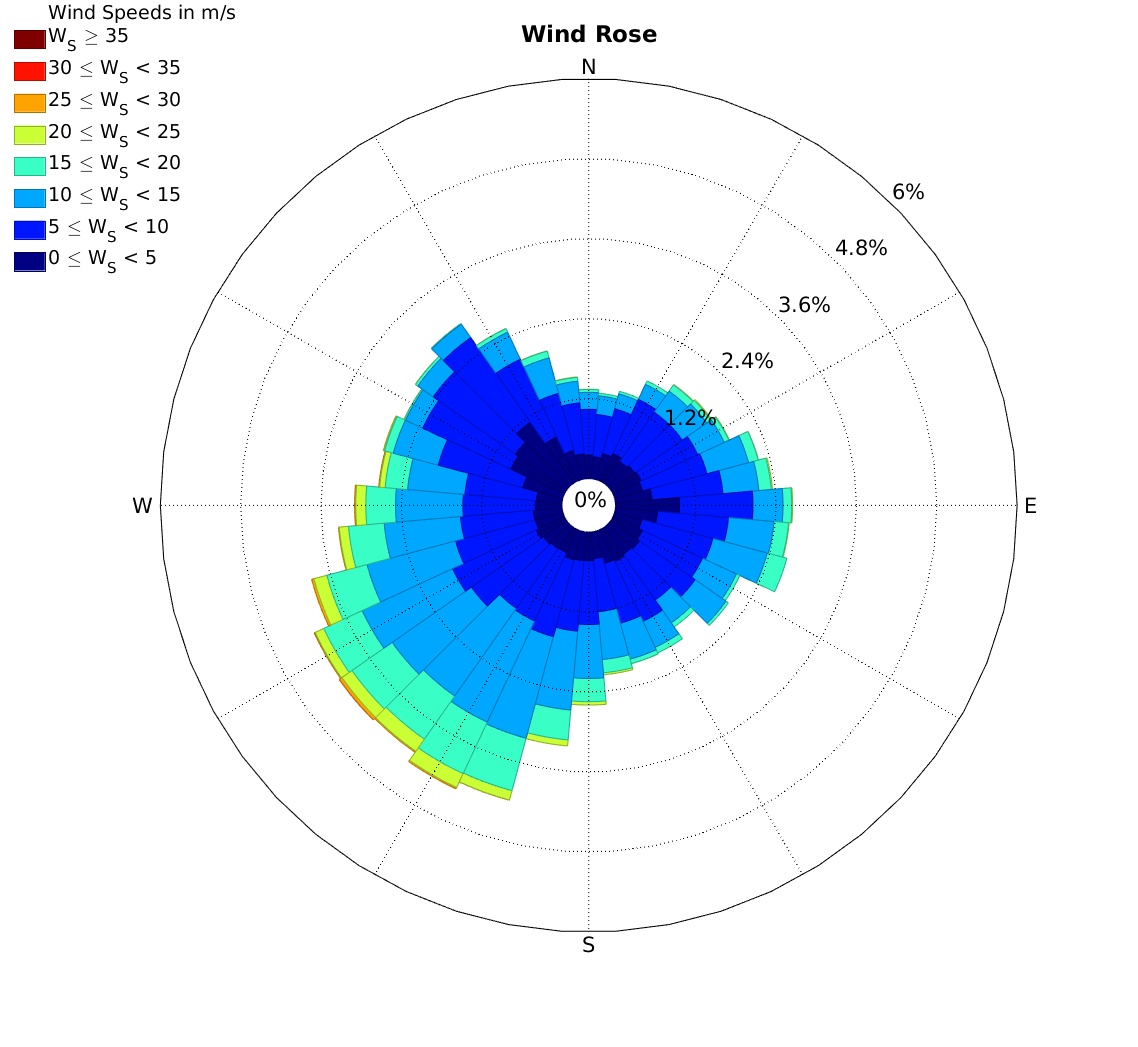
\includegraphics[width=0.3\linewidth]{../../figures/WindRose_Fino1.png}
\caption{Wind Rose of FINO 1}
\end{figure}

\end{frame}
\begin{frame}
	\frametitle{Wind Roses}
\begin{figure}[htbp]
	\begin{center}
		\begin{minipage}[t]{0.4\linewidth}
			\centering
			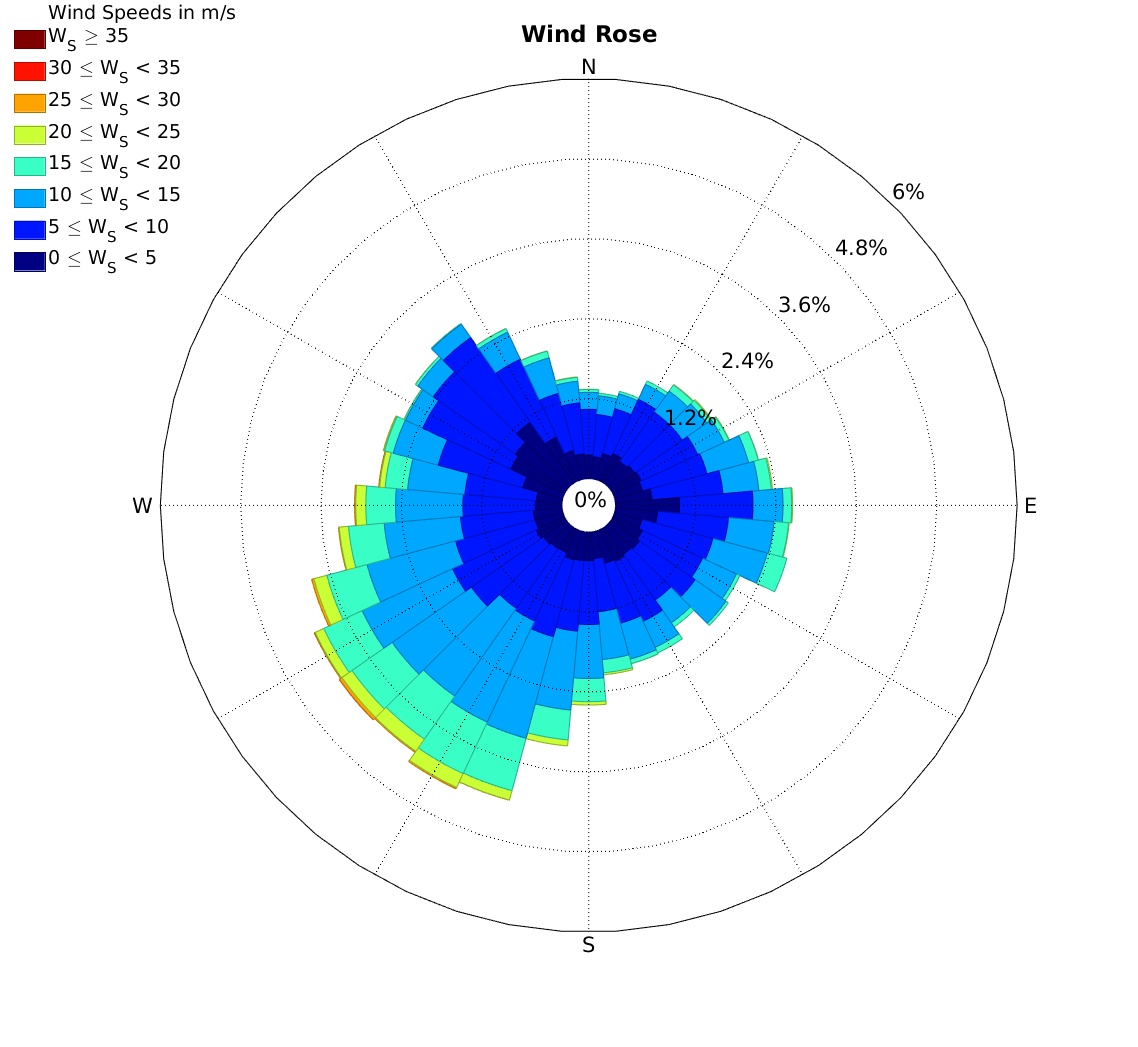
\includegraphics[width=\linewidth]{../../figures/WindRose_Fino1.png}
			\caption{Wind Rose of FINO 1}
			\label{label 1}
		\end{minipage}
		\qquad
		\pause
		\begin{minipage}[t]{0.45\linewidth}
			\centering
			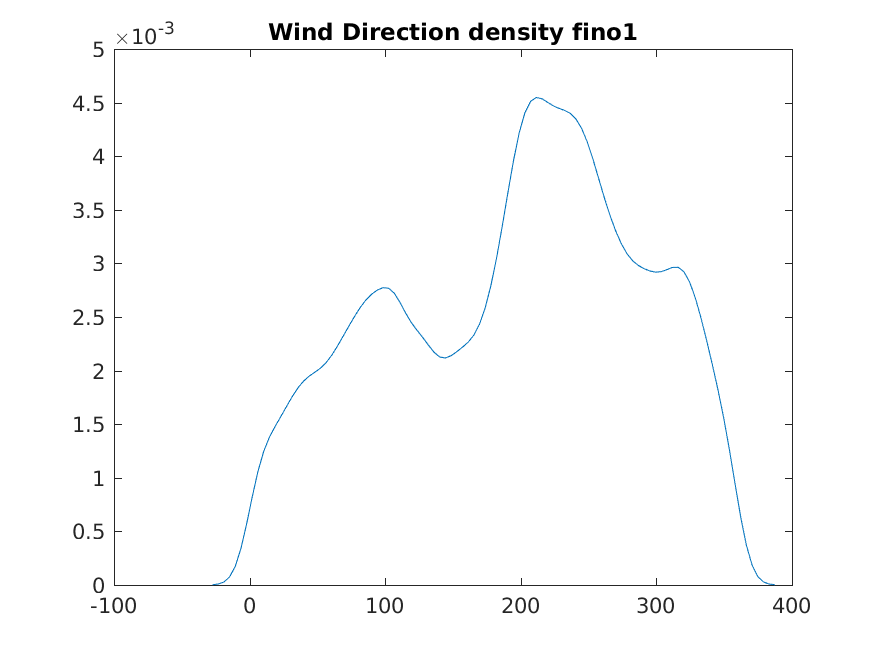
\includegraphics[width=\linewidth]{../../figures/Validation_WindRose_Fino1.png}
			\caption{Validation of Wind Rose}
			\label{label 2}
		\end{minipage}
	\end{center}
\end{figure}
\end{frame}

\begin{frame}
	\frametitle{Wind Roses}
\begin{figure}[htbp]
	\begin{center}
		\begin{minipage}[t]{0.4\linewidth}
			\centering
			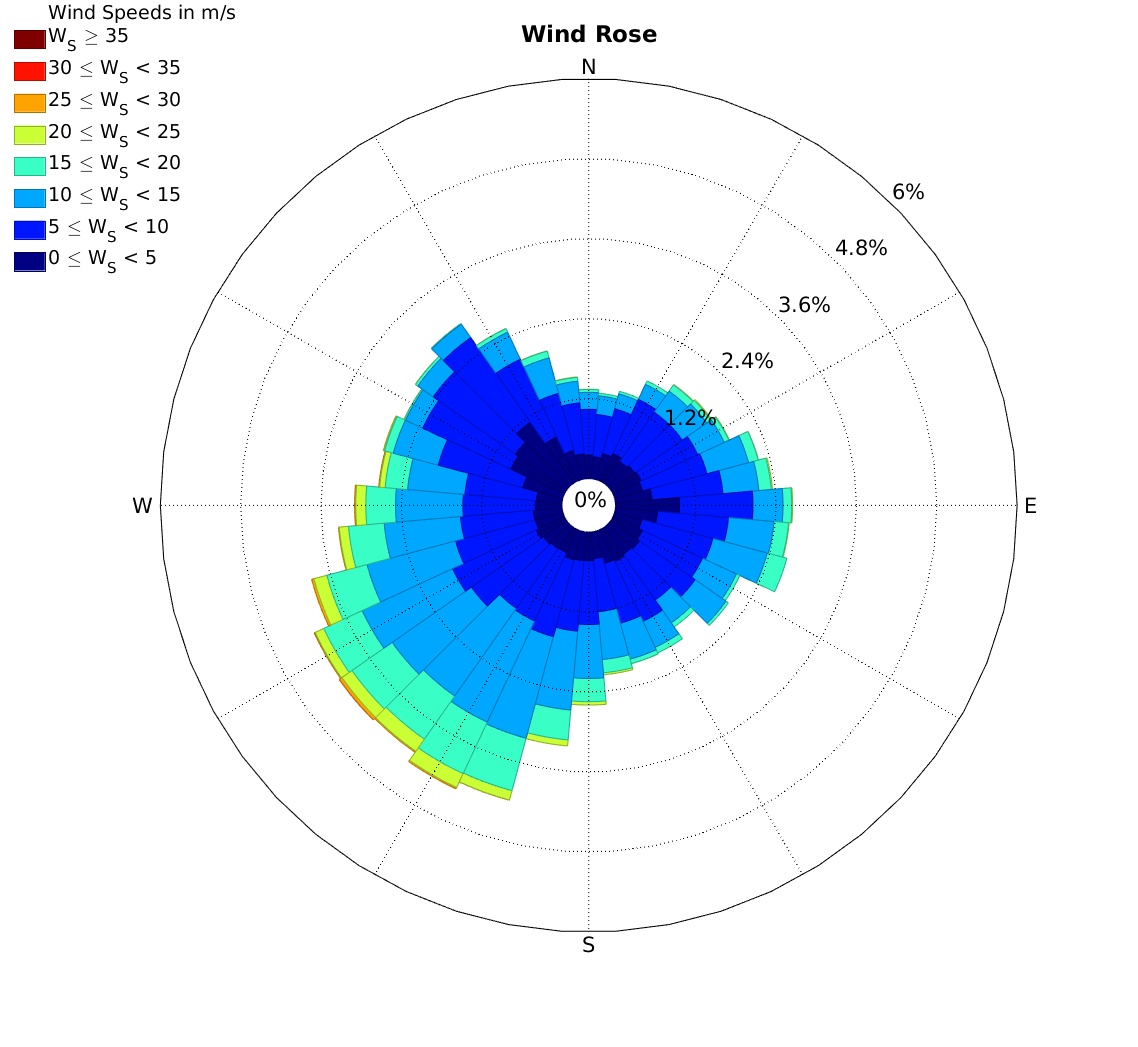
\includegraphics[width=\linewidth]{../../figures/WindRose_Fino1.png}
			\caption{Wind Rose of FINO 1}
			\label{label 1}
		\end{minipage}
		\qquad
		\begin{minipage}[t]{0.4\linewidth}
			\centering
			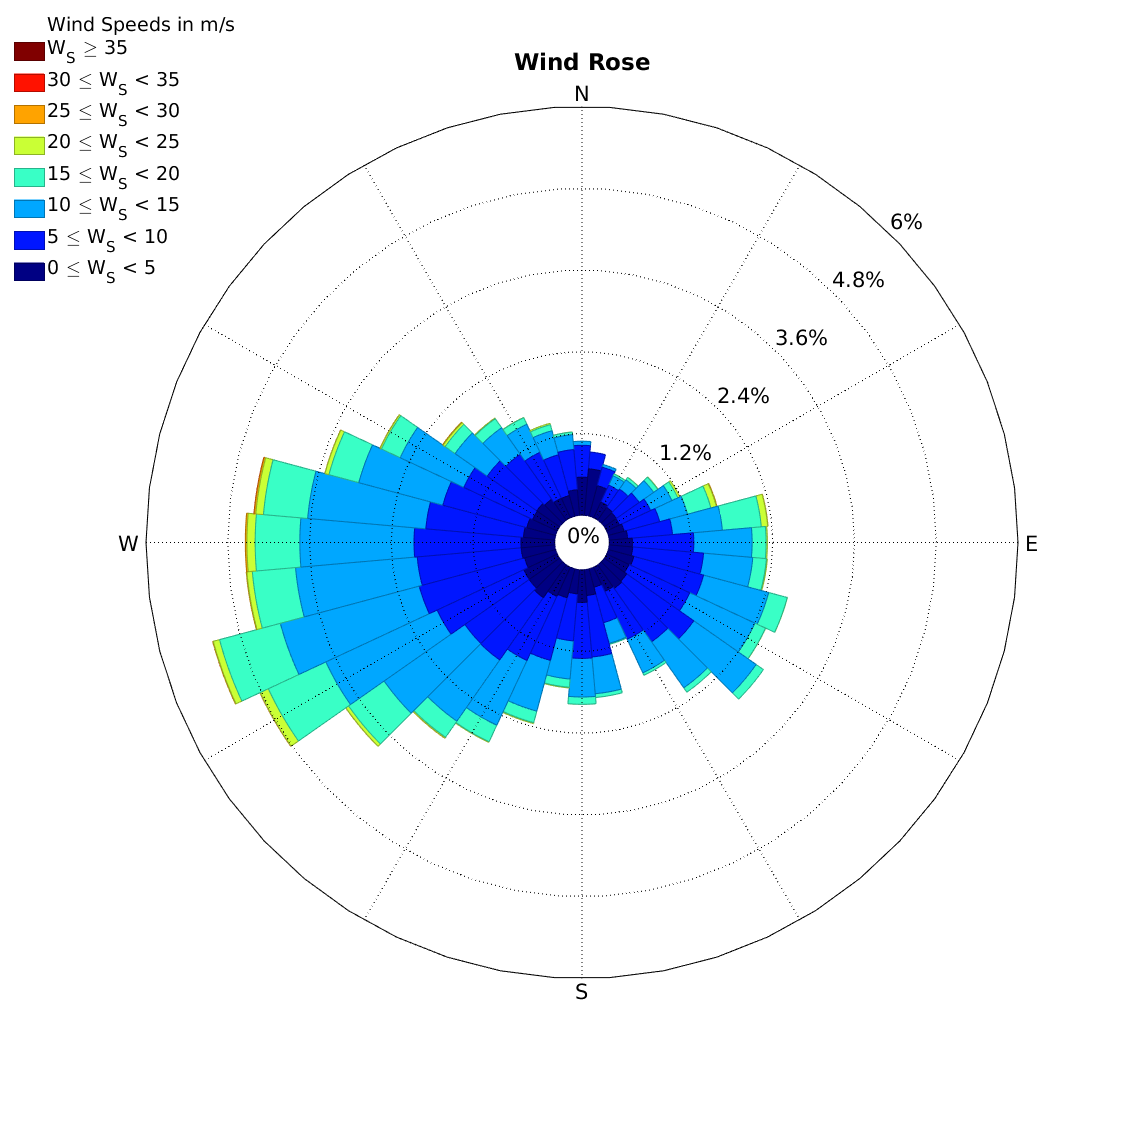
\includegraphics[width=\linewidth]{../../figures/WindRose_Fino2.png}
			\caption{Wind Rose of FINO 2}
			\label{label 2}
		\end{minipage}
	\end{center}
\end{figure}
\end{frame}
\begin{frame}
\frametitle{Differences}
\begin{figure}[H]
\centering
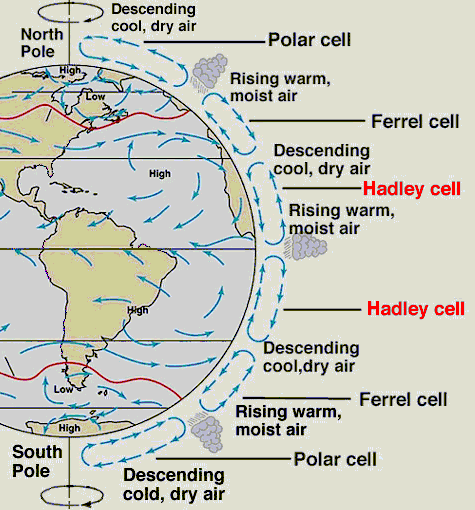
\includegraphics[width=0.5\linewidth]{../../figures/Ferrel_cell.png}
\caption{Geographical Distribution of Winds}
\label{fig:weatherpattern}
\end{figure}
\end{frame}


\begin{frame}
\frametitle{Differences}
\begin{figure}[H]
\centering
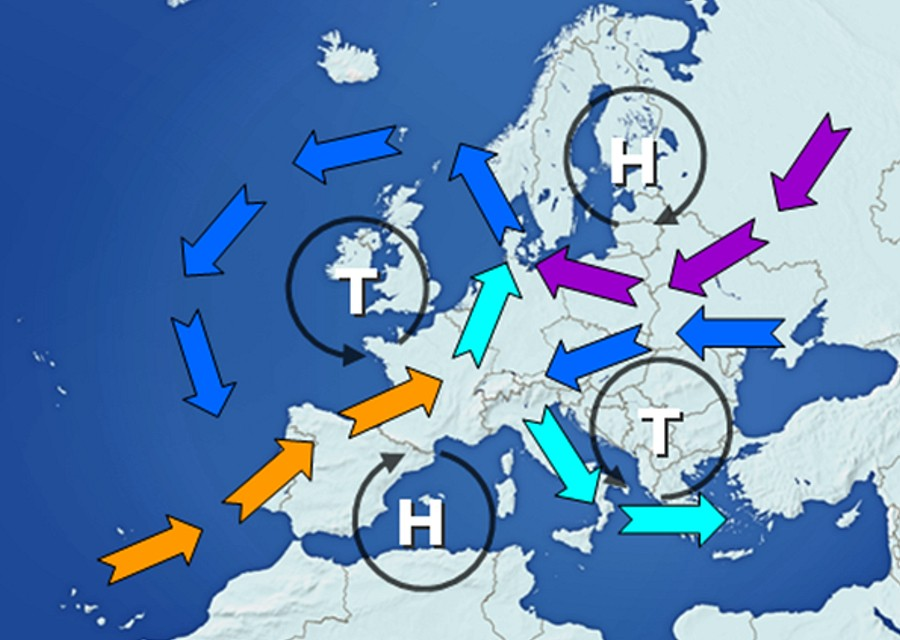
\includegraphics[width=0.7\linewidth]{../../figures/warm_air_advection.png}
\caption{Typical weather pattern over Europe}
\label{fig:weatherpattern}
\end{figure}
\end{frame}


\begin{frame}
\frametitle{Obstacles}
\begin{figure}[H]
\centering
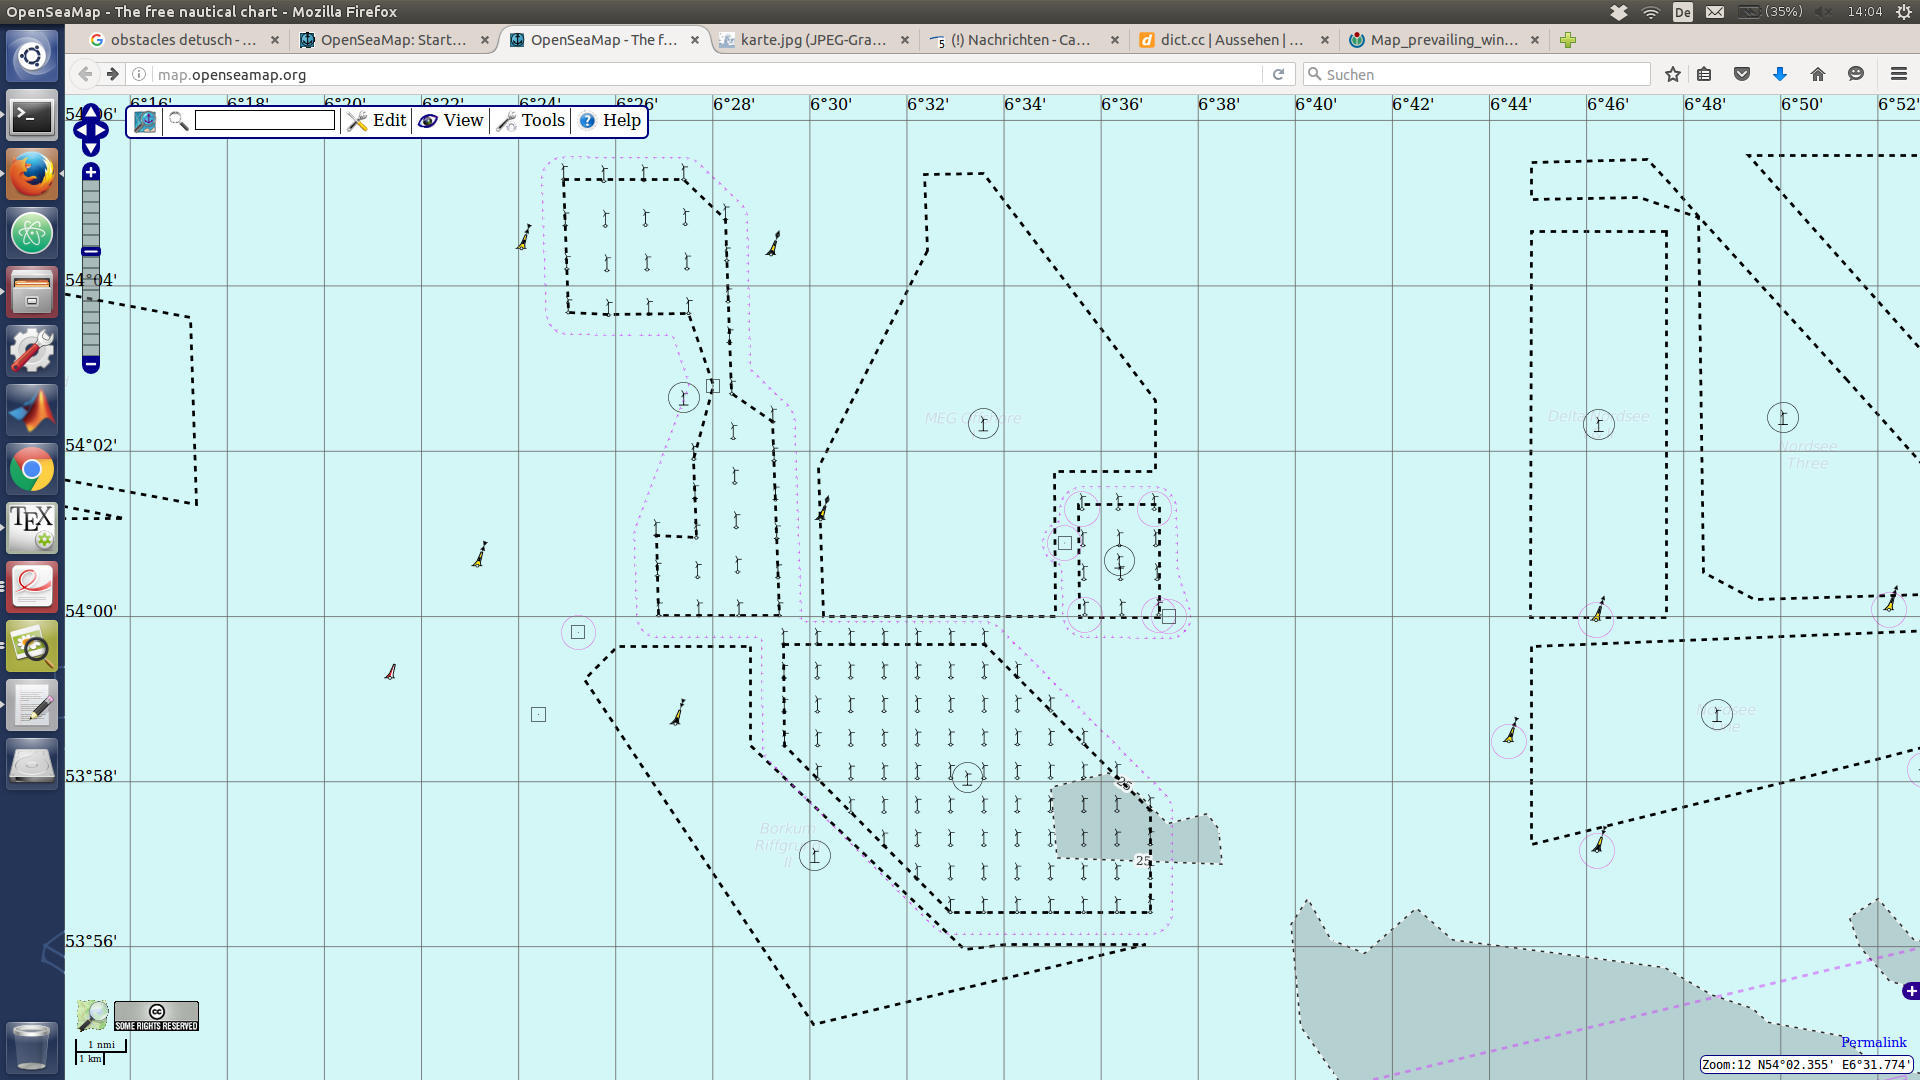
\includegraphics[width=0.8\linewidth]{../../figures/fino1.png}
\caption{Location of FINO 1}
\label{fig:fino1}
\end{figure} 
\end{frame}
\section{Weibull distribution}
%%%%%%%%%%%% End of content %%%%%%%%%%%%

\section*{Ende}

	\begin{frame}
		\frametitle{Ende}
		\begin{center}
			\Large \textbf{Vielen Dank für Ihre Aufmerksamkeit!}\\
			\large \textbf{Haben Sie Fragen?}\\
		\end{center}
	\end{frame}
	
	% Black frame to separte appendix
	\setbeamercolor{background canvas}{bg=black}
	\begin{frame}[plain]
	\end{frame}
	\setbeamercolor{background canvas}{bg=white}

%%%%%%%%%%%% Start of appendix %%%%%%%%%%%% 

%%%%%%%%%%%% End of appendix %%%%%%%%%%%%

\end{document}